\documentclass[9pt]{IEEEtran}

\usepackage[english]{babel}
\usepackage{graphicx}
\usepackage{epstopdf}
\usepackage{fancyhdr}
\usepackage{amsmath}
\usepackage{amsthm}
\usepackage{amssymb}
\usepackage{url}
\usepackage{array}
\usepackage{textcomp}
\usepackage{listings}
\usepackage{hyperref}
\usepackage{xcolor}
\usepackage{colortbl}
\usepackage{float}
\usepackage{gensymb}
\usepackage{longtable}
\usepackage{supertabular}
\usepackage{multicol}
\usepackage[utf8x]{inputenc}
\usepackage[T1]{fontenc}
\usepackage{lmodern}
\input{glyphtounicode}
\pdfgentounicode=1

\graphicspath{{./figures/}}
\DeclareGraphicsExtensions{.pdf,.png,.jpg,.eps}

\hyphenation{op-tical net-works semi-conduc-tor trig-gs}

\title{\vspace{0ex}
Parallel Histogram Equalization Using CUDA}

\author{First-name Last-name\vspace{-4.0ex}}

\begin{document}

\maketitle

\section{Introduction}
This project implements a parallel histogram equalization algorithm for colour images using CUDA. Histogram equalization is a widely used technique to improve the contrast in images by redistributing the luminance values. In our solution, the image is first converted from RGB to YUV colour space so that the luminance (Y) component can be processed independently. We then compute the histogram and cumulative distribution function (CDF) of the Y channel, create a lookup table (LUT), and apply it to obtain the equalized image before converting back to RGB.

The implementation consists of a sequential CPU version, a baseline parallel CUDA version, and an optimized bonus version that uses shared memory for partial histogram computation. Our objective was to offload the entire algorithm to the GPU, minimize data transfers, and reduce atomic contention to achieve significant speed-ups.

\section{Experiments}
We evaluated the implementations on images of sizes: 720x480, 1024x768, 1920x1200, 3840x2160, and 7680x4320. Each experiment was repeated 7 times. The average execution times (in milliseconds) for each approach are summarized in Table~\ref{tab:avg_times}.

\begin{table}[H]
\centering
\begin{tabular}{|c|c|c|c|}
\hline
Image Size & Sequential & Parallel & Bonus \\ \hline
720x480   & 14.60 ms  & 0.74 ms  & 0.47 ms  \\ \hline
1024x768  & 29.25 ms  & 1.00 ms  & 0.75 ms  \\ \hline
1920x1200 & 80.46 ms  & 3.14 ms  & 1.61 ms  \\ \hline
3840x2160 & 274.34 ms & 7.75 ms  & 4.04 ms  \\ \hline
7680x4320 & 989.65 ms & 31.53 ms & 15.23 ms \\ \hline
\end{tabular}
\caption{Average execution times for each implementation.}
\label{tab:avg_times}
\end{table}

The speed-up factors, calculated as the ratio of sequential to parallel execution time, are shown in Table~\ref{tab:speedups}. For larger images the baseline parallel version achieves a speed-up of up to 35\(\times\) and the bonus version up to 68\(\times\).

\begin{table}[H]
\centering
\begin{tabular}{|c|c|c|}
\hline
Image Size & Parallel Speed-Up & Bonus Speed-Up \\ \hline
720x480   & 19.7\(\times\)   & 31.0\(\times\) \\ \hline
1024x768  & 29.3\(\times\)   & 39.3\(\times\) \\ \hline
1920x1200 & 25.6\(\times\)   & 49.9\(\times\) \\ \hline
3840x2160 & 35.4\(\times\)   & 67.9\(\times\) \\ \hline
7680x4320 & 31.4\(\times\)   & 65.0\(\times\) \\ \hline
\end{tabular}
\caption{Speed-up factors relative to the sequential implementation.}
\label{tab:speedups}
\end{table}

Figure~\ref{fig:speedup} illustrates the speed-up achieved by both parallel versions. The plot clearly shows the increasing benefit of parallelization as image resolution grows.

\begin{figure}[H]
    \centering
    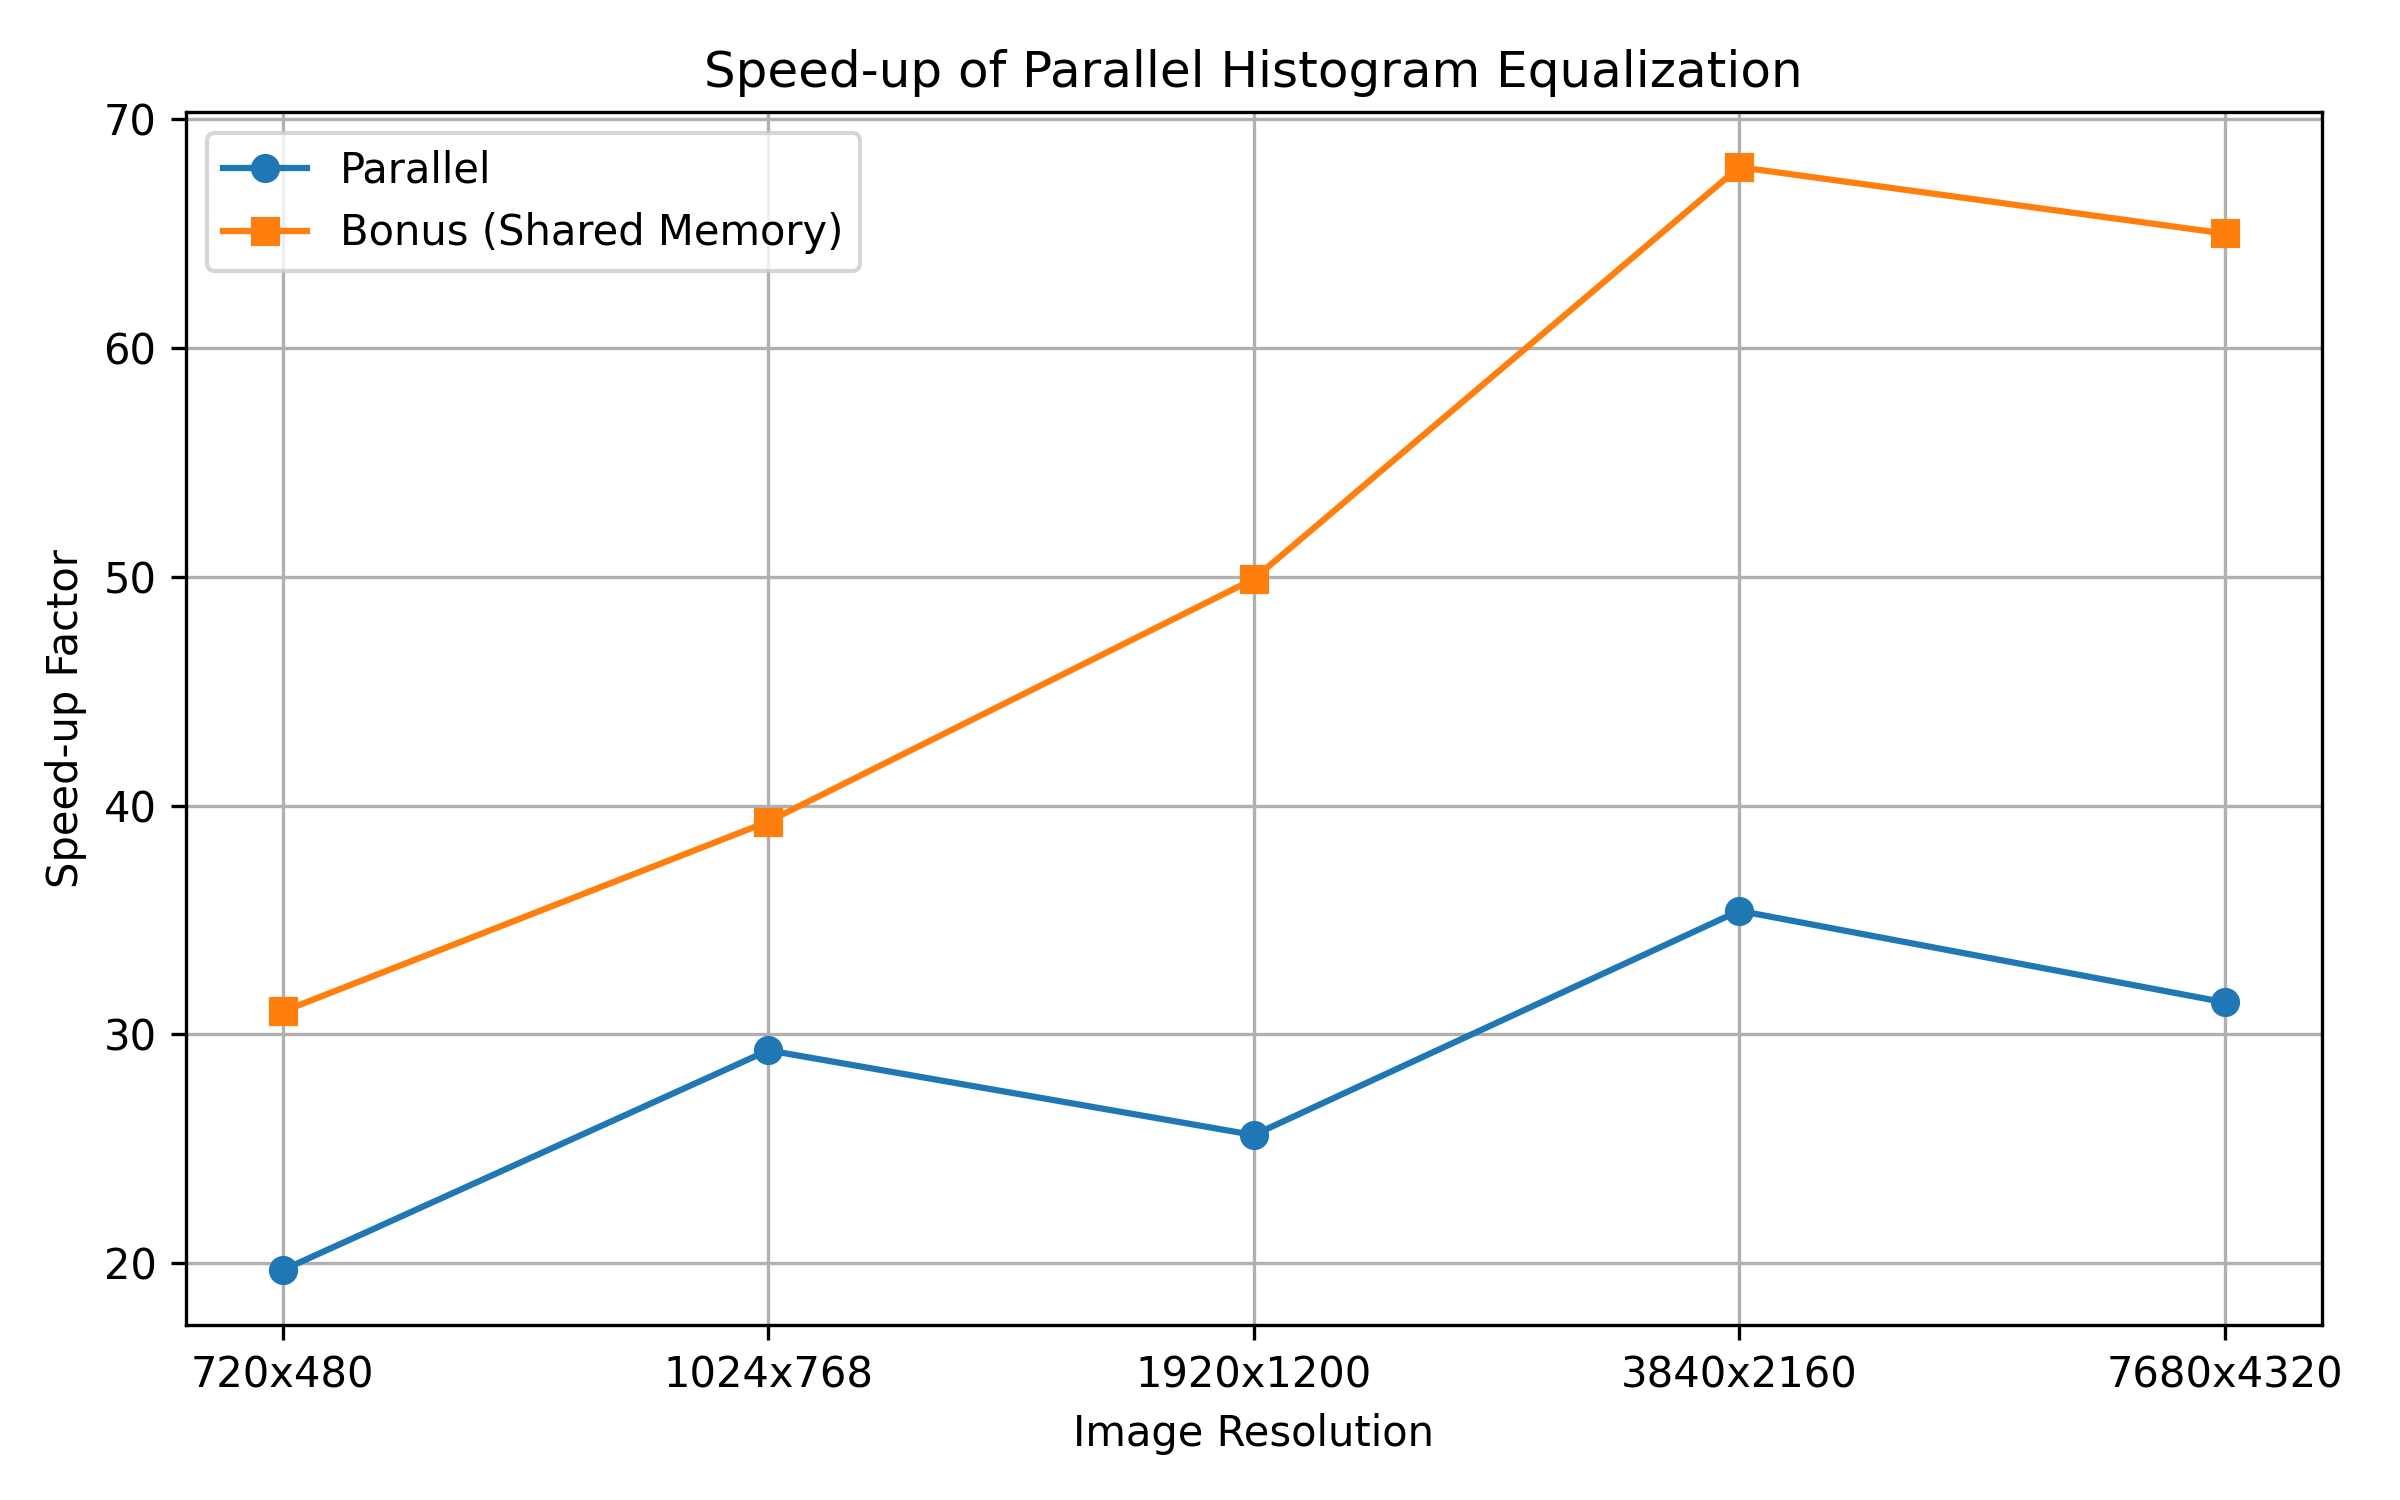
\includegraphics[width=0.9\columnwidth]{speedup.png}
    \caption{Speed-up comparison of the parallel and bonus implementations relative to the sequential version.}
    \label{fig:speedup}
\end{figure}

\subsection*{Discussion}
The baseline parallel implementation shows significant improvement over the sequential version, largely due to the independent processing of pixels and effective use of CUDA atomic operations. However, the bonus version, which employs shared memory for computing partial histograms, reduces atomic contention and further improves performance, particularly for high-resolution images. Variations in sequential timings (e.g., an outlier in the 7680x4320 case) are likely due to system overhead and data transfer variability. Future work could further optimize kernel configurations and memory usage.

\section{Conclusion}
The parallel histogram equalization algorithm implemented using CUDA demonstrates substantial speed-ups compared to a sequential approach. The bonus version, leveraging shared memory optimizations, performs even better, especially on larger images. While the method works well for scientific imaging tasks, further improvements in atomic operation handling and memory synchronization may yield additional performance gains.

\bibliographystyle{IEEEtran}
\bibliography{bibliography}

\end{document}
